%%%%%%%%%%%%%%%%%%%%%%%%%%%%%%%%%%%%%%%%%
% Full Length Professional CV
% LaTeX Template
% Version 2.0 (13/6/20)
%
% Original author:
% Sreedhar Unnikrishnakurup 
%
% Important note:
% This template requires the my_cv.cls file to be in the same directory as the .tex file. The my_cv.cls file provides the resume style used for structuring the document. THe publication.bib file is needed for adding the publication list
%
%%%%%%%%%%%%%%%%%%%%%%%%%%%%%%%%%%%%%%%%%

%----------------------------------------------------------------------------------------
%	PACKAGES AND OTHER DOCUMENT CONFIGURATIONS
%----------------------------------------------------------------------------------------

\documentclass{my_cv}% Use the custom my_cv.cls style
\begin{document}
\title{CV}
\author{Sreedhar Unnikrishnakurup}
\begin{minipage}{0.8\textwidth}
\begingroup
\let\center\flushleft
\let\endcenter\endflushleft
\maketitle
\endgroup
\end{minipage}
\begin{minipage}{0.1\textwidth}
\begin{tikzpicture}[remember picture,overlay]
\clip ($(current page text area.north east)!0.01!(current page text area.south east)!-7.4!(current page text area.north west)$)
  circle (2.1cm) node {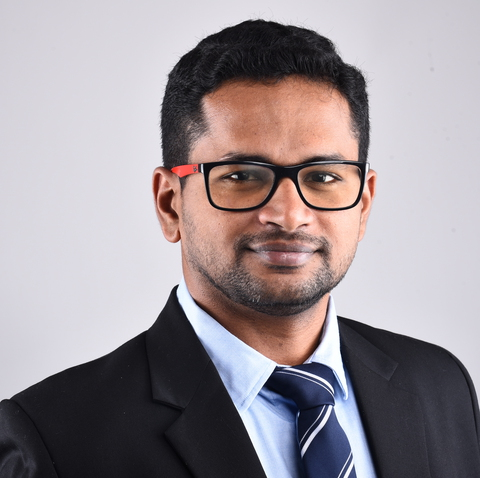
\includegraphics[width=2.3\linewidth]{mypic2}};
\end{tikzpicture}
%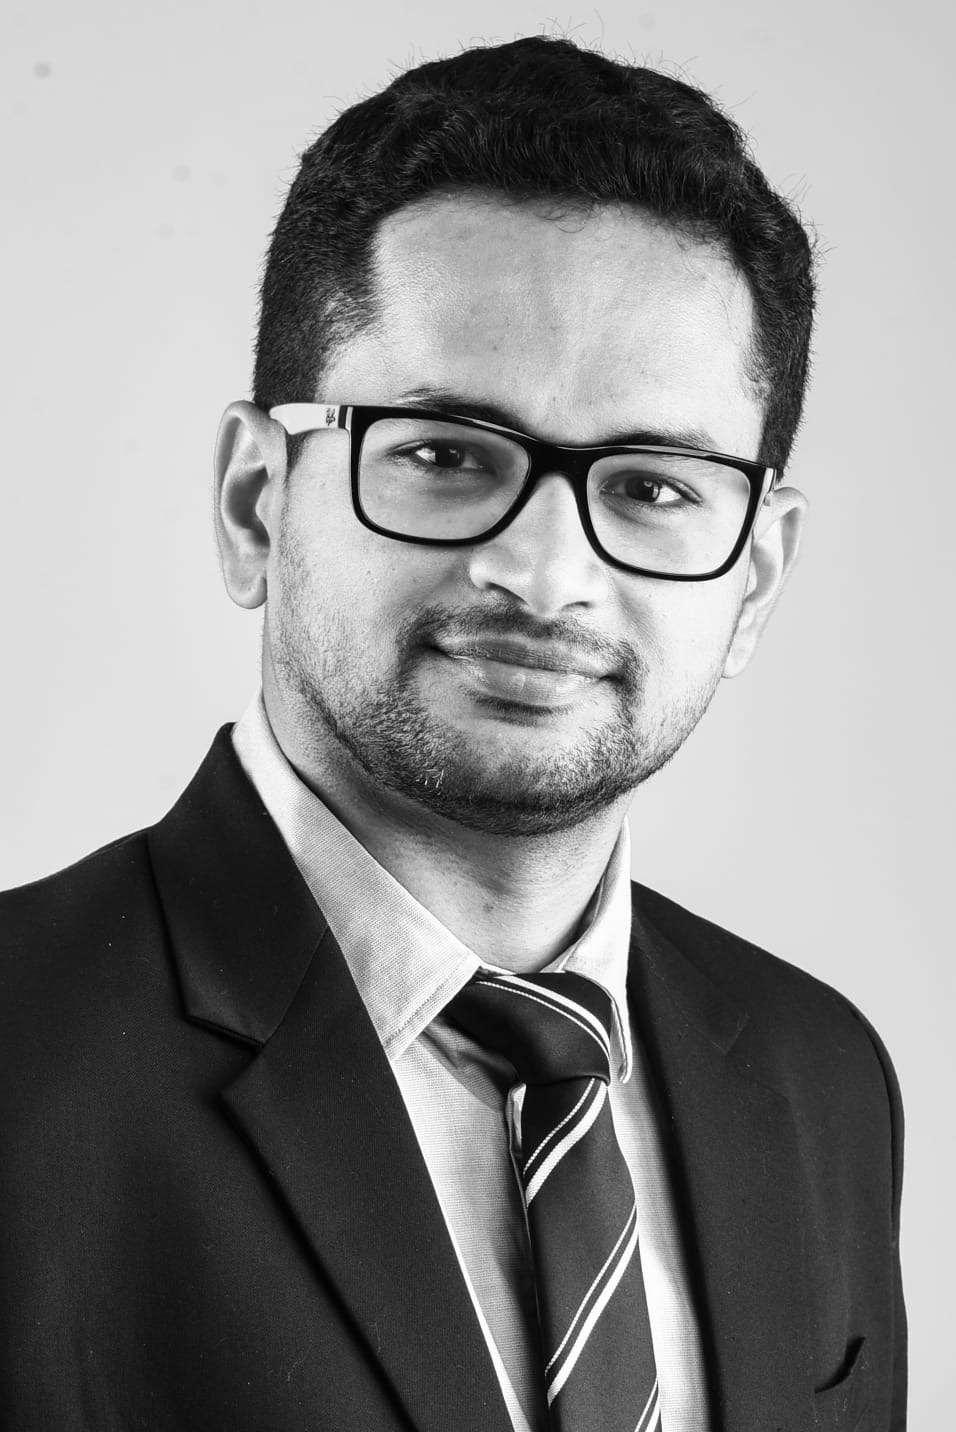
\includegraphics[width=8em]{mypic}
\end{minipage}
\vspace{1.5em}
%-------------------------------------------------------------
%	HIGHLIGHTS
%-------------------------------------------------------------
\section{Faits saillants}
\vspace{1.0em}
\begin{itemize}[leftmargin=0.15in]
\setlength\itemsep{-0.1em}
\color{mygray}
\item Plus de 11 ans d'expérience en thermographie infrarouge (IRT), spécifiquement en IRT pulsée pour l'inspection de l'épaisseur des revêtements, inspection des composites utilisant l'IRT pulsée, l'IRT de verrouillage et l'IRT par induction, l'IRT laser pour l'inspection des fissures, et les simulations numériques des méthodes de test de thermographie.
\item Doctorat de l'Université de Montpellier 2, France en génie du soudage, simulation multiphysique et analyse inverse pour l'optimisation multiparamétrique.
\item Master de l'Institut Indien de Technologie (IIT) Madras en surveillance en ligne de la qualité des soudures utilisant l'IRT.
\item \textbf{Certification de niveau 1} en thermographie infrarouge, plusieurs années d'expérience dans la manipulation des caméras FLIR et expertise en analyse d'images thermiques. 16 publications dans des journaux et 32 présentations de conférences.
\end{itemize}
%-------------------------------------------------------------
%	WORK EXPERIENCE SECTION
%-------------------------------------------------------------
\section{Expérience Professionnelle}
\vspace{1.0em}
\subsection{Scientifique}
\subsubsection{\href{https://www.a-star.edu.sg/imre}{Institut de Recherche en Ingénierie et Matériaux (IMRE), A*STAR}}
\datedsubsection{Nov 2021--En cours}{Singapour}
\begin{itemize}[leftmargin=0.15in]
\setlength\itemsep{-0.1em}
\color{mygray}
\item Applications avancées de thermographie infrarouge non destructrice : IRT pulsée, IRT par induction, et IRT laser.
\item Caractérisation des dommages et inhomogénéités dans les systèmes composites renforcés par fibres (CFRP, GFRP) et métaux.
\item Évaluation de la porosité des revêtements, détection de fissures dans les composants métalliques même sous peinture avec IRT par induction, modélisation et simulation des techniques IRT et utilisation de l'IA pour une meilleure détection des défauts.
\end{itemize}
{\color{mygray1} \hdashrule[0.1ex]{18.8cm}{0.2mm}{1mm}}
\subsection{Chercheur Postdoctoral}
\subsubsection{\href{https://www.cnde.in/}{Centre pour l'Évaluation Non Destructive (CNDE), IIT Madras}}
\datedsubsection{Mai 2018 - Sep 2021}{Chennai, Inde}
\begin{itemize}[leftmargin=0.15in]
\setlength\itemsep{-0.1em}
\color{mygray}
\item Application du test IRT non destructif pour l'inspection de l'épaisseur des revêtements barrières thermiques et validation à l'aide de tests THz-TDS et par courants de Foucault.
\item Inspection de composites utilisant IRT à chauffage par induction.
\item Inspection de fissures dans des billettes d'acier à des températures élevées à l'aide de IRT assistée par laser.
\item Développement d'imagerie radiographique avancée assistée par IA et reconnaissance automatique des défauts pour les soudures critiques et les matériaux à haute énergie.
\item Investigation numérique de la diffusion thermique anisotrope dans les microstructures polycristallines et composites.
\end{itemize}
{\color{mygray1} \hdashrule[0.1ex]{18.8cm}{0.2mm}{1mm}}
%{\color{mygray} \rule{\linewidth}{0.5mm} }
\subsection{Membre de la Cohorte BA3}
\subsubsection{\href{https://www.joinef.com/}{Entrepreneur First}}
\datedsubsection{Février 2020 - Mai 2020}{Bangalore, Inde}
\begin{itemize}[leftmargin=0.15in]
\setlength\itemsep{-0.1em}
\color{mygray}
\item Exploration de plusieurs solutions technologiques intéressantes, étude du marché, validation de la technologie, interaction avec les clients et recherche sur les prototypes.
\item Les idées sur lesquelles nous avons travaillé incluent la détection et le signalement de médicaments contrefaits ou de qualité compromise, en utilisant un dispositif d'imagerie hyperspectrale basé sur l'IA, mobile et économique.
\end{itemize}
{\color{mygray1} \hdashrule[0.1ex]{18.8cm}{0.2mm}{1mm}}
\subsection{Chercheur Postdoctoral}
\subsubsection{\href{https://www.bam.de/Navigation/DE/Home/home.html}{Groupe NDT 8.7, Institut Fédéral pour la Recherche et les Tests sur les Matériaux (BAM)}}
\datedsubsection{Janvier 2016 - Juin 2017}{Berlin, Allemagne}
\begin{itemize}[leftmargin=0.15in]
\setlength\itemsep{-0.1em}
\color{mygray}
\item Développement de simulations informatiques pour étudier les tests thermographiques actifs pour la détection de défauts dans les composites.
\item Tests IRT pulsés, en verrouillage de phase, et par chauffage par paliers sur des composites renforcés de fibres.
\item Optimisation et validation de la thermographie active comme technique NDE non-contact, rapide et à champ complet pour les tests quantitatifs sur les structures en PRF.
\end{itemize}
{\color{mygray1} \hdashrule[0.1ex]{18.8cm}{0.2mm}{1mm}}
\subsection{Chercheur Invité}
\subsubsection{\href{https://innowacje.zut.edu.pl/cooperationoffer/electromagnetic-methods-non-destructive-testing}{Groupe de Recherche sur les Méthodes Électromagnétiques de Contrôle Non Destructif, Université de Technologie de Poméranie Occidentale (ZUT)}}
\datedsubsection{Janvier 2015 - Juin 2015}{Szczecin, Pologne}
\begin{itemize}[leftmargin=0.15in]
\setlength\itemsep{-0.1em}
\color{mygray}
\item Imagerie terahertz et analyse temporelle pour l'identification de défauts matériels dans les pales d'éoliennes composites.
\item Thermographie infrarouge active pour l'identification de défauts dans les matériaux composites - Investigations numériques des effets de puits de chaleur dans l'inspection infrarouge des composites.
\end{itemize}
{\color{mygray1} \hdashrule[0.1ex]{18.8cm}{0.2mm}{1mm}}
\subsection{Chercheur Postdoctoral de l'Institut}
\subsubsection{\href{https://www.cnde.in/}{Centre pour l'Évaluation Non Destructive (CNDE), IIT Madras}}
\datedsubsection{Septembre 2014 - Décembre 2015}{Chennai, Inde}
\begin{itemize}[leftmargin=0.15in]
\setlength\itemsep{-0.1em}
\color{mygray}
\item Modélisation numérique de la diffusion thermique microstructurale et de la propagation d'ondes ultrasonores dans les matériaux polycristallins.
\item Surveillance du processus de soudage CMT utilisant la thermographie IR.
\item Thermographie laser en ligne pour la surveillance en ligne de billettes d'acier afin de prédire les fissures de surface formées lors du refroidissement non uniforme.
\end{itemize}
{\color{mygray1} \hdashrule[0.1ex]{18.8cm}{0.2mm}{1mm}}
\subsection{Associé de Recherche}
\subsubsection{\href{https://www.cnde.in/}{Centre pour l'Évaluation Non Destructive (CNDE), IIT Madras}}
\datedsubsection{Avril 2007 - Décembre 2008}{Chennai, Inde}
\begin{itemize}[leftmargin=0.15in]
\setlength\itemsep{-0.1em}
\color{mygray}
\item Développement de la surveillance en ligne de la qualité des soudures pour les réservoirs de propergol liquide AA2219 utilisant l'imagerie thermique infrarouge et la radiographie aux rayons X.
\item Développement d'un modèle d'éléments finis pour la prédiction des profils de température pendant le soudage.
\end{itemize}
%-------------------------------------------------------------
%	EDUCATION SECTION
%-------------------------------------------------------------
\section{Éducation}
\vspace{2em}
\subsection{\href{https://adum.fr/as/ed/cv.pl?mat=39446&site=adumR} {Doctorat en Mécanique et Génie Civil}}
\subsubsection{\faInstitution \hspace{0.2em} \href{https://www.umontpellier.fr/en/}{Université de Montpellier 2 (UM2)}}
\datedsubsection{2011 - 2014}{Montpellier, France}
\begin{itemize}[leftmargin=0.15in]
\setlength\itemsep{-0.1em}
\color{mygray}
\item Sujet de thèse : Identification de la forme du bain de soudure utilisant la modélisation multiphysique et des expériences
\end{itemize}
{\color{mygray1} \hdashrule[0.1ex]{18.8cm}{0.2mm}{1mm}}
\subsection{M.S. en Génie Mécanique}
\subsubsection{\faInstitution \hspace{0.2em} \href{https://www.iitm.ac.in/}{Institut Indien de Technologie Madras}}
\datedsubsection{2008 - 2010}{Chennai, Inde}
\begin{itemize}[leftmargin=0.15in]
\setlength\itemsep{-0.1em}
\color{mygray}
\item Sujet de thèse : Surveillance en ligne de la qualité du soudage utilisant l'imagerie thermique infrarouge
\item Moyenne Générale Cumulative de 8 sur 10
\end{itemize}
{\color{mygray1} \hdashrule[0.1ex]{18.8cm}{0.2mm}{1mm}}
\subsection{Licence en Génie Mécanique}
\subsubsection{\faInstitution \hspace{0.2em} \href{https://www.ieindia.org/webui/iei-home.aspx}{Institut des Ingénieurs de l'Inde}}
\datedsubsection{2002 - 2006}{Kottayam, Inde}
\begin{itemize}[leftmargin=0.15in]
\setlength\itemsep{-0.1em}
\color{mygray}
\item Moyenne Générale Cumulative de 6.94 sur 10
\end{itemize}
%-------------------------------------------------------------
%	Publication
%-------------------------------------------------------------
\section{Publication}
\vspace{1em}
\nobibliography{publication}
\begin{itemize}
    \item 16 publications dans des revues et 12 présentations en conférences.
    \item La liste complète des publications est disponible à l'URL : \href{https://bit.ly/30BlL05}{https://bit.ly/30BlL05}
\end{itemize}

%---------------------------------------------------------------
%	                 SKILLS SECTION
%-------------------------------------------------------------
\section{Compétences}
\vspace{1em}
\begin{minipage}{0.35\textwidth}
\cvSkill{5}    MATLAB \\           
\cvSkill{4}  Python \\
   
\end{minipage}
\begin{minipage}{0.35\textwidth}
\cvSkill{5}   FEM: COMSOL \\
\cvSkill{4}   \LaTeX \\

\end{minipage}
\begin{minipage}{0.35\textwidth}
\cvSkill{5}   Deep learning \\
\cvSkill{4}   Machine Learning \\

\end{minipage}

%-------------------------------------------------------------
%	                 Certifications and Courses
%-------------------------------------------------------------
\section{Certifications et Cours}
\vspace{1em}
\begin{itemize}[leftmargin=0.15in]
\setlength\itemsep{-0.1em}
\color{mygray}
\item[\faCertificate] Fondamentaux de la Gestion de Projet par EPM. Délivré en octobre 2022
\item[\faCertificate] Thermographie Infrarouge Niveau 1 par le Centre de Formation Infrarouge. Délivré en mai 2022
\item[\faCertificate] Apprentissage Profond, une spécialisation de 5 cours par deeplearning.ai sur Coursera. Certificat de spécialisation obtenu le 23 septembre 2018
\end{itemize}

%-------------------------------------------------------------
%	                 Languages
%-------------------------------------------------------------
\section{Langues}
\vspace{1em}
\noindent
\begin{minipage}{0.4\textwidth}
\begin{itemize}
\setlength\itemsep{0.0em}
\item[] Anglais  \hspace{0.5em} \cvSkill{5} 
\item[] Allemand  \hspace{0.2em} \cvSkill{3} 
\item[] Français  \hspace{0.8em} \cvSkill{2}
\end{itemize}
\end{minipage}
%seconde colonne
\begin{minipage}{0.4\textwidth}
\begin{itemize}
\setlength\itemsep{0.0em}
\item[] Malayalam  \hspace{0.5em} \cvSkill{5} 
\item[] Hindi      \hspace{2.9em} \cvSkill{2} 
\item[] Tamil      \hspace{2.9em} \cvSkill{3}
\end{itemize}
\end{minipage}
\vspace{2em}
%---------------------------------------------------------------
%	Reference
%----------------------------------------------------------------
\section{Références}
\vspace{1em}
\begin{minipage}{0.6\textwidth}
\subsubsection{Prof. Krishnan Balasubramaniam} 
\faAt \hspace{0.2em} \href{mailto:balas@iitm.ac.in}{balas@iitm.ac.in} \\
\hspace{0.5em} \faInstitution \hspace{0.2em} \href{http://iitm.irins.org/profile/50968}{Department of Mechanical Engineering, IIT Madras}
\vspace{1.5em}
\subsubsection{Dr. Fabien Soulie} 
\faAt \hspace{0.2em} \href{mailto:fabien.soulie@umontpellier.fr}{fabien.soulie@umontpellier.fr}\\ \hspace{0.2em}\faInstitution \hspace{0.2em}  \href{http://www.lmgc.univ-montp2.fr/spip.php?page=pageperso&nom=SOULIE&prenom=Fabien&lang=fr}{UM2/LMGC}
\vspace{1em}
\end{minipage}
\begin{minipage}{0.6\textwidth}
\subsubsection{Dr. Sebastien Rouquette} 
\faAt \hspace{0.2em} \href{mailto:sebastien.rouquette@umontpellier.fr}{sebastien.rouquette@umontpellier.fr}\\ \faInstitution \hspace{0.2em} \href{http://www.lmgc.univ-montp2.fr/spip.php?page=pageperso&nom=ROUQUETTE&prenom=Sebastien&lang=fr}{UM2/LMGC}
\vspace{1.2em}
\subsubsection{Dr. C. V. Krishnamurthy} 
\faAt \hspace{0.2em} \href{mailto:cvkm@iitm.ac.in}{cvkm@iitm.ac.in} \\
\faInstitution \hspace{0.2em} \href{http://iitm.irins.org/profile/61936}{Department of Physics, IIT Madras}
\end{minipage}
%-------------------------------------------------------------
\end{document}




\begin{comment}
\subsubsection{Dr. C. V. Krishnamurthy} 
\faAt \hspace{0.2em} \href{mailto:cvkm@iitm.ac.in}{cvkm@iitm.ac.in} \\
\faInstitution \hspace{0.2em} \href{http://iitm.irins.org/profile/61936}{Department of Physics, IIT Madras}
\subsubsection{}
\vspace{4.8em}
\end{comment}